\chapter{Process Analysis}

%As this project have mainly been focused on learning new topics on our own, it is important to also talk about the outcome of the specialization period. This chapter will go over the goals of the project and whether or not we feel these goals have been achieved.

\section{Project Planning}
\label{ProjectPlanning}
As we have already mentioned in section \ref{WorkProcess} we used the kanbanflow tool to manage our tasks and work flow for this project. All red tasks is programming/product oriented, where the yellow is report/documentation related. The plan did change slightly a few times due to new acquired knowledge on the topic and there by forcing us to change the schedule slightly. Each change have always be made after an iteration have ended as changing the schedule midway through an iteration is often wrong to do when working in iterations.

We saw in section \ref{WorkProcess} how we initially planned out our project, but we did under estimate how much we could do in 3 weeks. Already after a week into the project period, had we already completed the most of the initial work of writing the introduction chapters as well as programming the most of the planned tasks for that iteration. We then began to take task from iteration 2 and slowly also empty out the second iteration and at the end of our first iteration we ended up with the schedule seen in \figref{fig:afteritration1}.

\begin{figure}[H]
	\includegraphics[width=1.0\linewidth]{img/afteriteration1}
	\centering
	\caption{Our schedule after iteration 1}
	\label{fig:afteritration1}
\end{figure}

As we in the schedule in \figref{fig:afteritration1} were almost a half iteration ahead we modified it to better match our current situation. As we in iteration 1 also got to look into some articles about procedural content generation, we got new knowledge about the topic, and realized that a few changes were necessary. As we can see in \figref{fig:BeforeIteration2}, we moved implementation from iteration 2 to iteration 3 and added a new task to iteration 2 about noise manipulation. We did also find out that the 2 task that was in progress were very huge and there were much more to them than we first though so we added in subtasks to both of them. By adding subtasks we also found that a few already existing tasks should be a subtask rather than a task for it self.

\begin{figure}[H]
	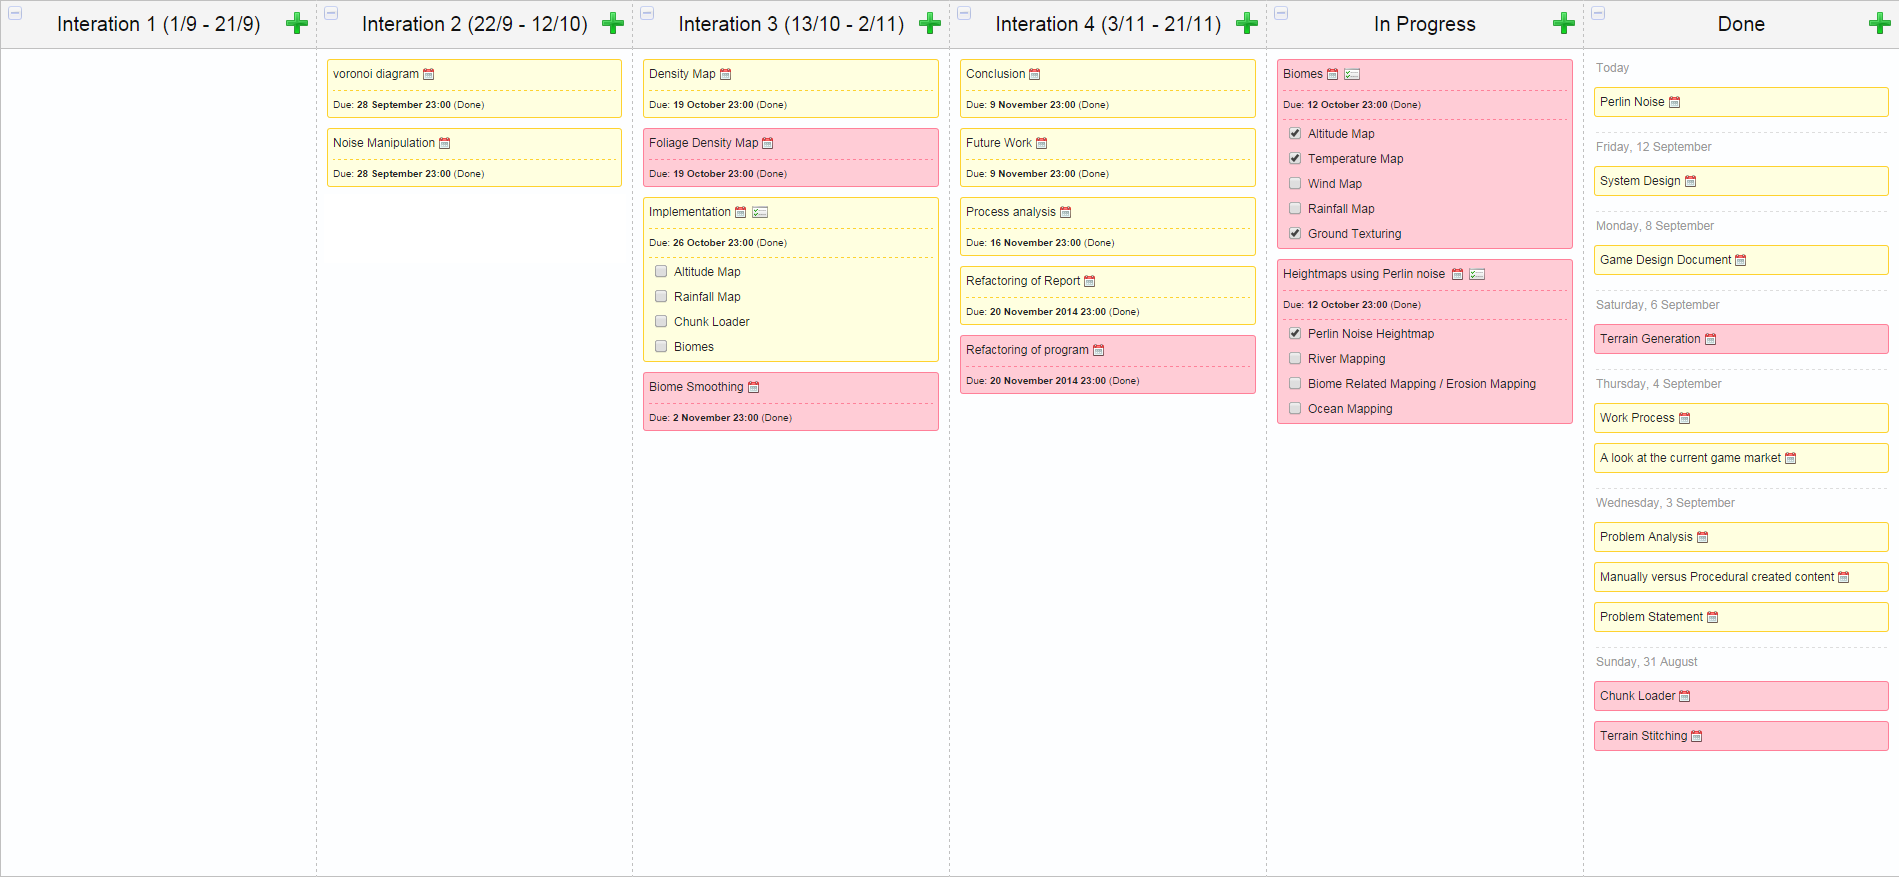
\includegraphics[width=1.0\linewidth]{img/BeforeIteration2}
	\centering
	\caption{Our schedule readjusted for iteration 2}
	\label{fig:BeforeIteration2}
\end{figure}

The reason behind we haven't added more than one new task to iteration 2 is due to the fact that the 2 current in progress tasks is very huge and we may need much longer time to certain subtask. Due to this we have decided to be vary with how many tasks we have for the second iteration.

\section{Work Process}



\section{Learning Outcome}



\section{Project Conclusion}

